\appendix  

\section{Įprasta tiekimo grandinė (Vertikaliai)}
\begin{figure}[H]
    \centering
    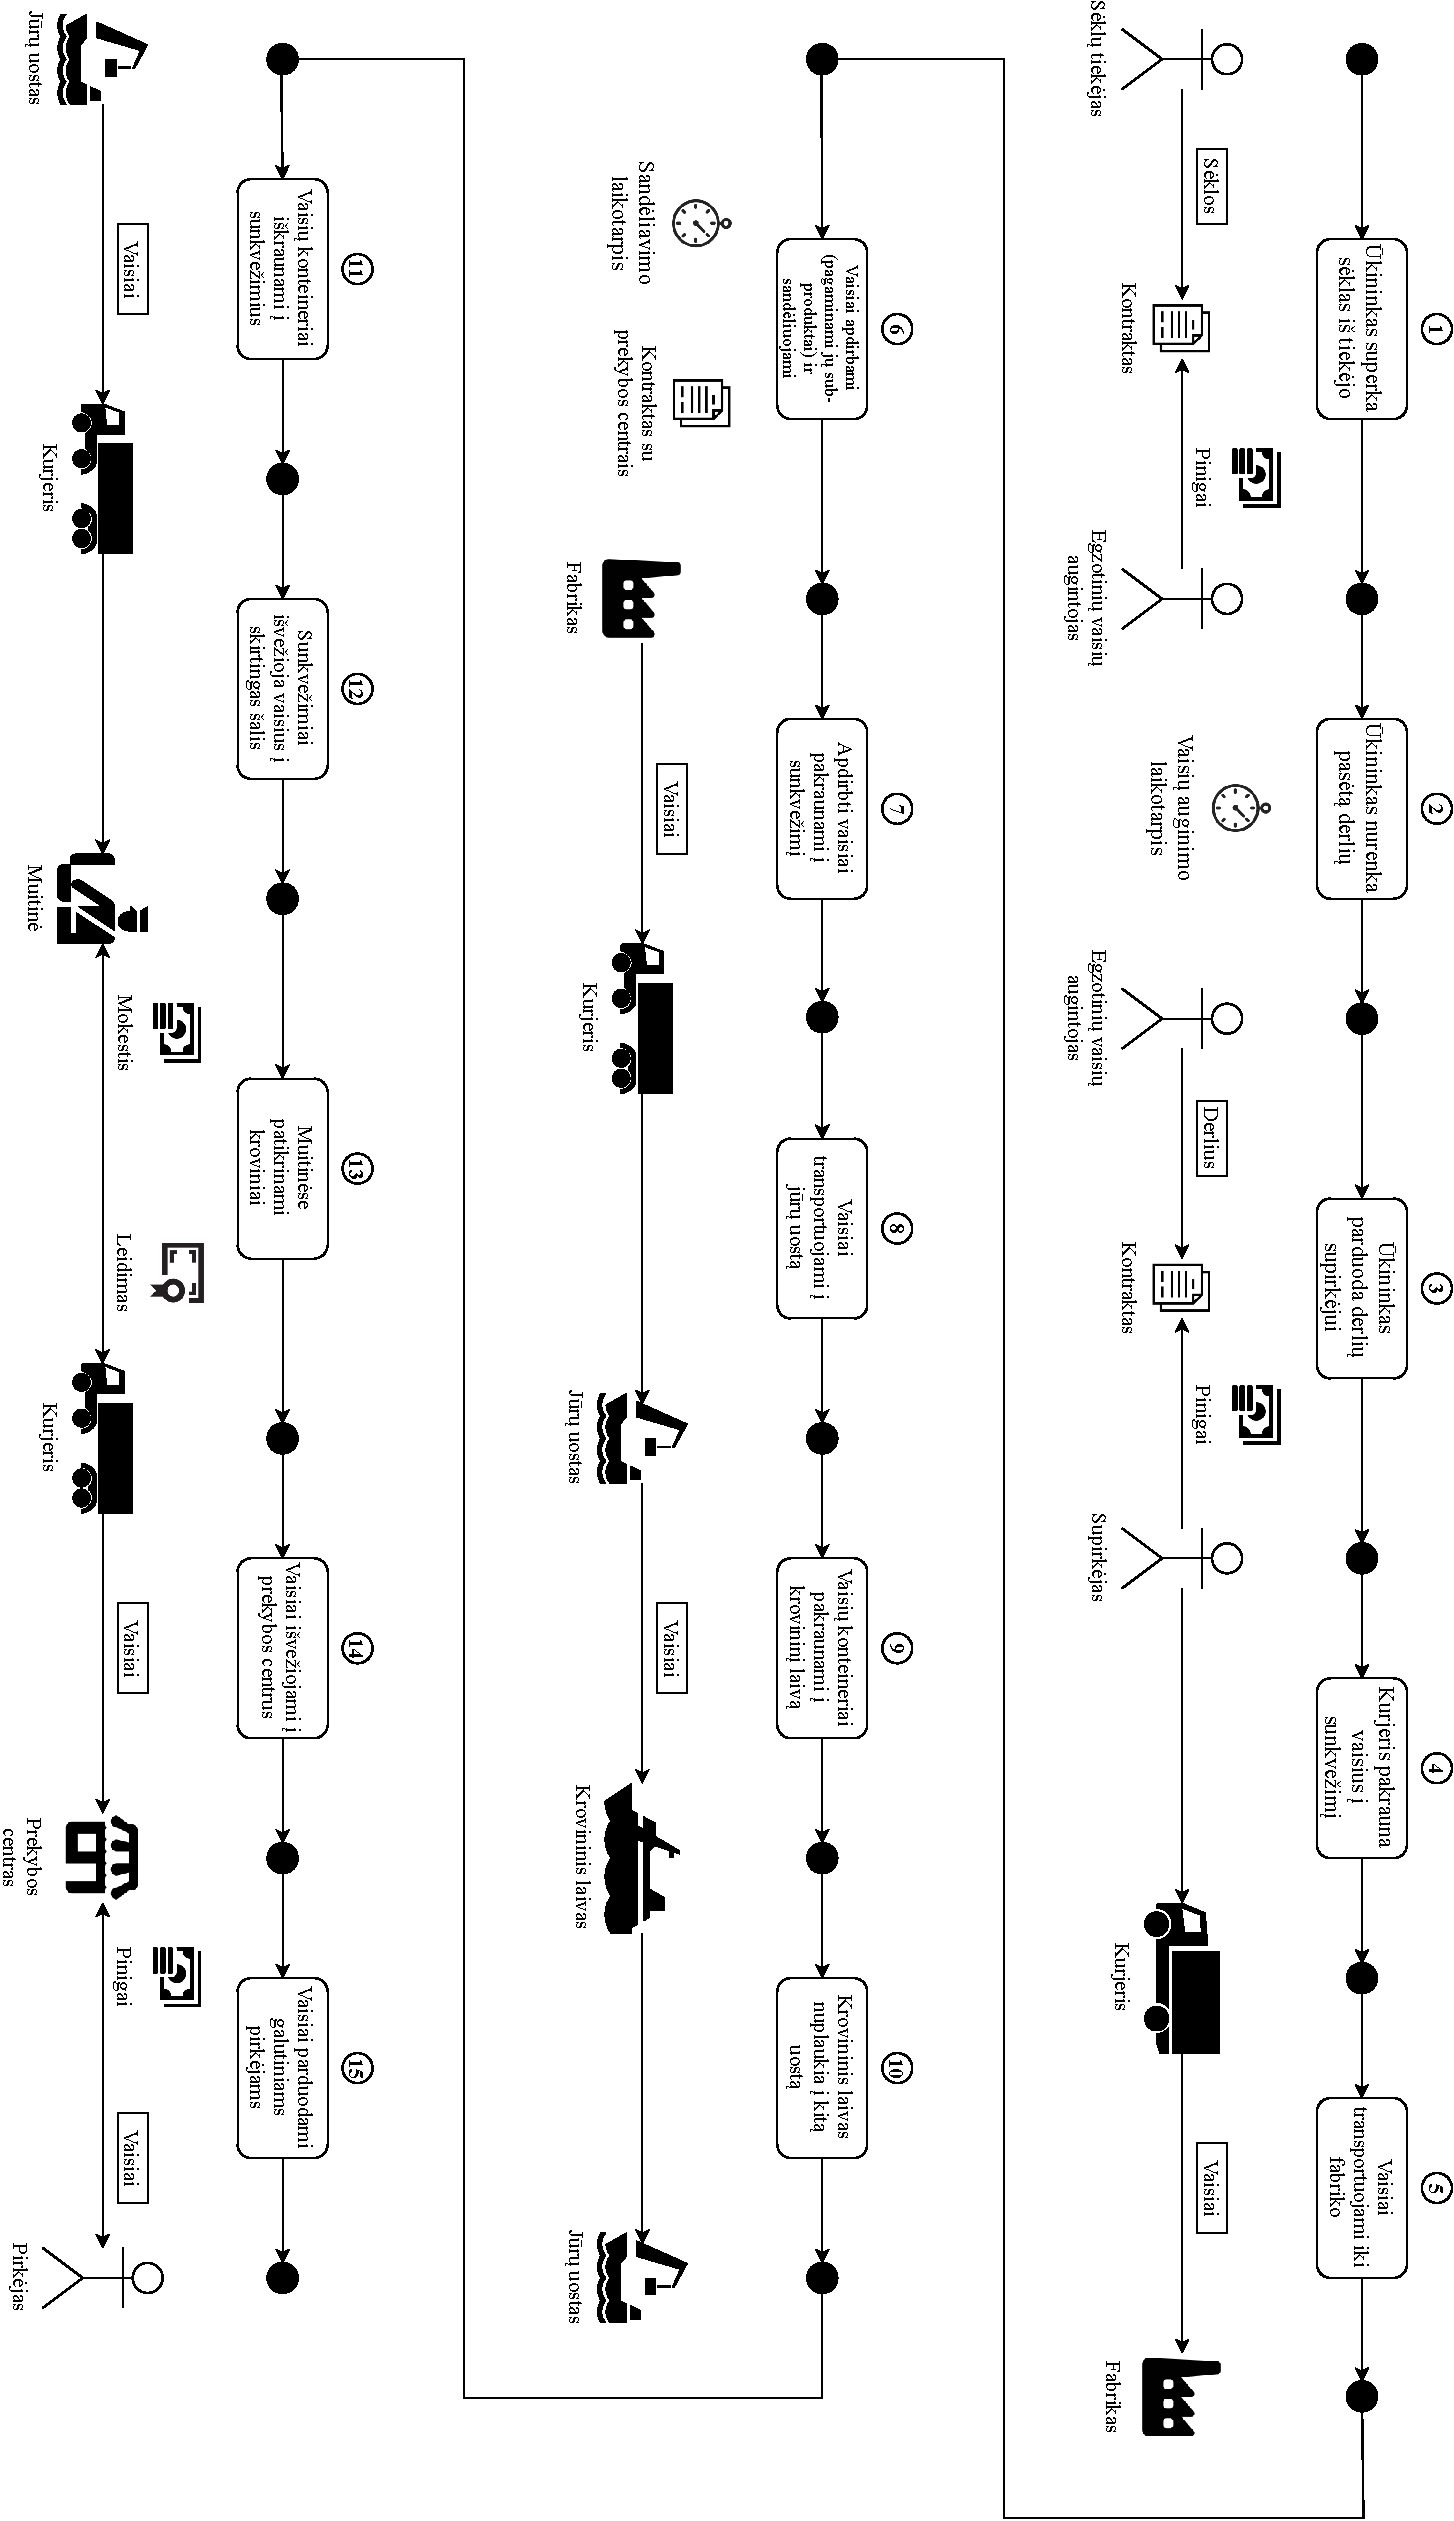
\includegraphics[scale=0.50]{images/supply-chain-vertical}
    \caption{Įprasta tiekimo grandinė (Horizontaliai)}
\end{figure}

\section{Įprasta tiekimo grandinė (Horizontaliai)}
\begin{figure}[H]
    \centering
    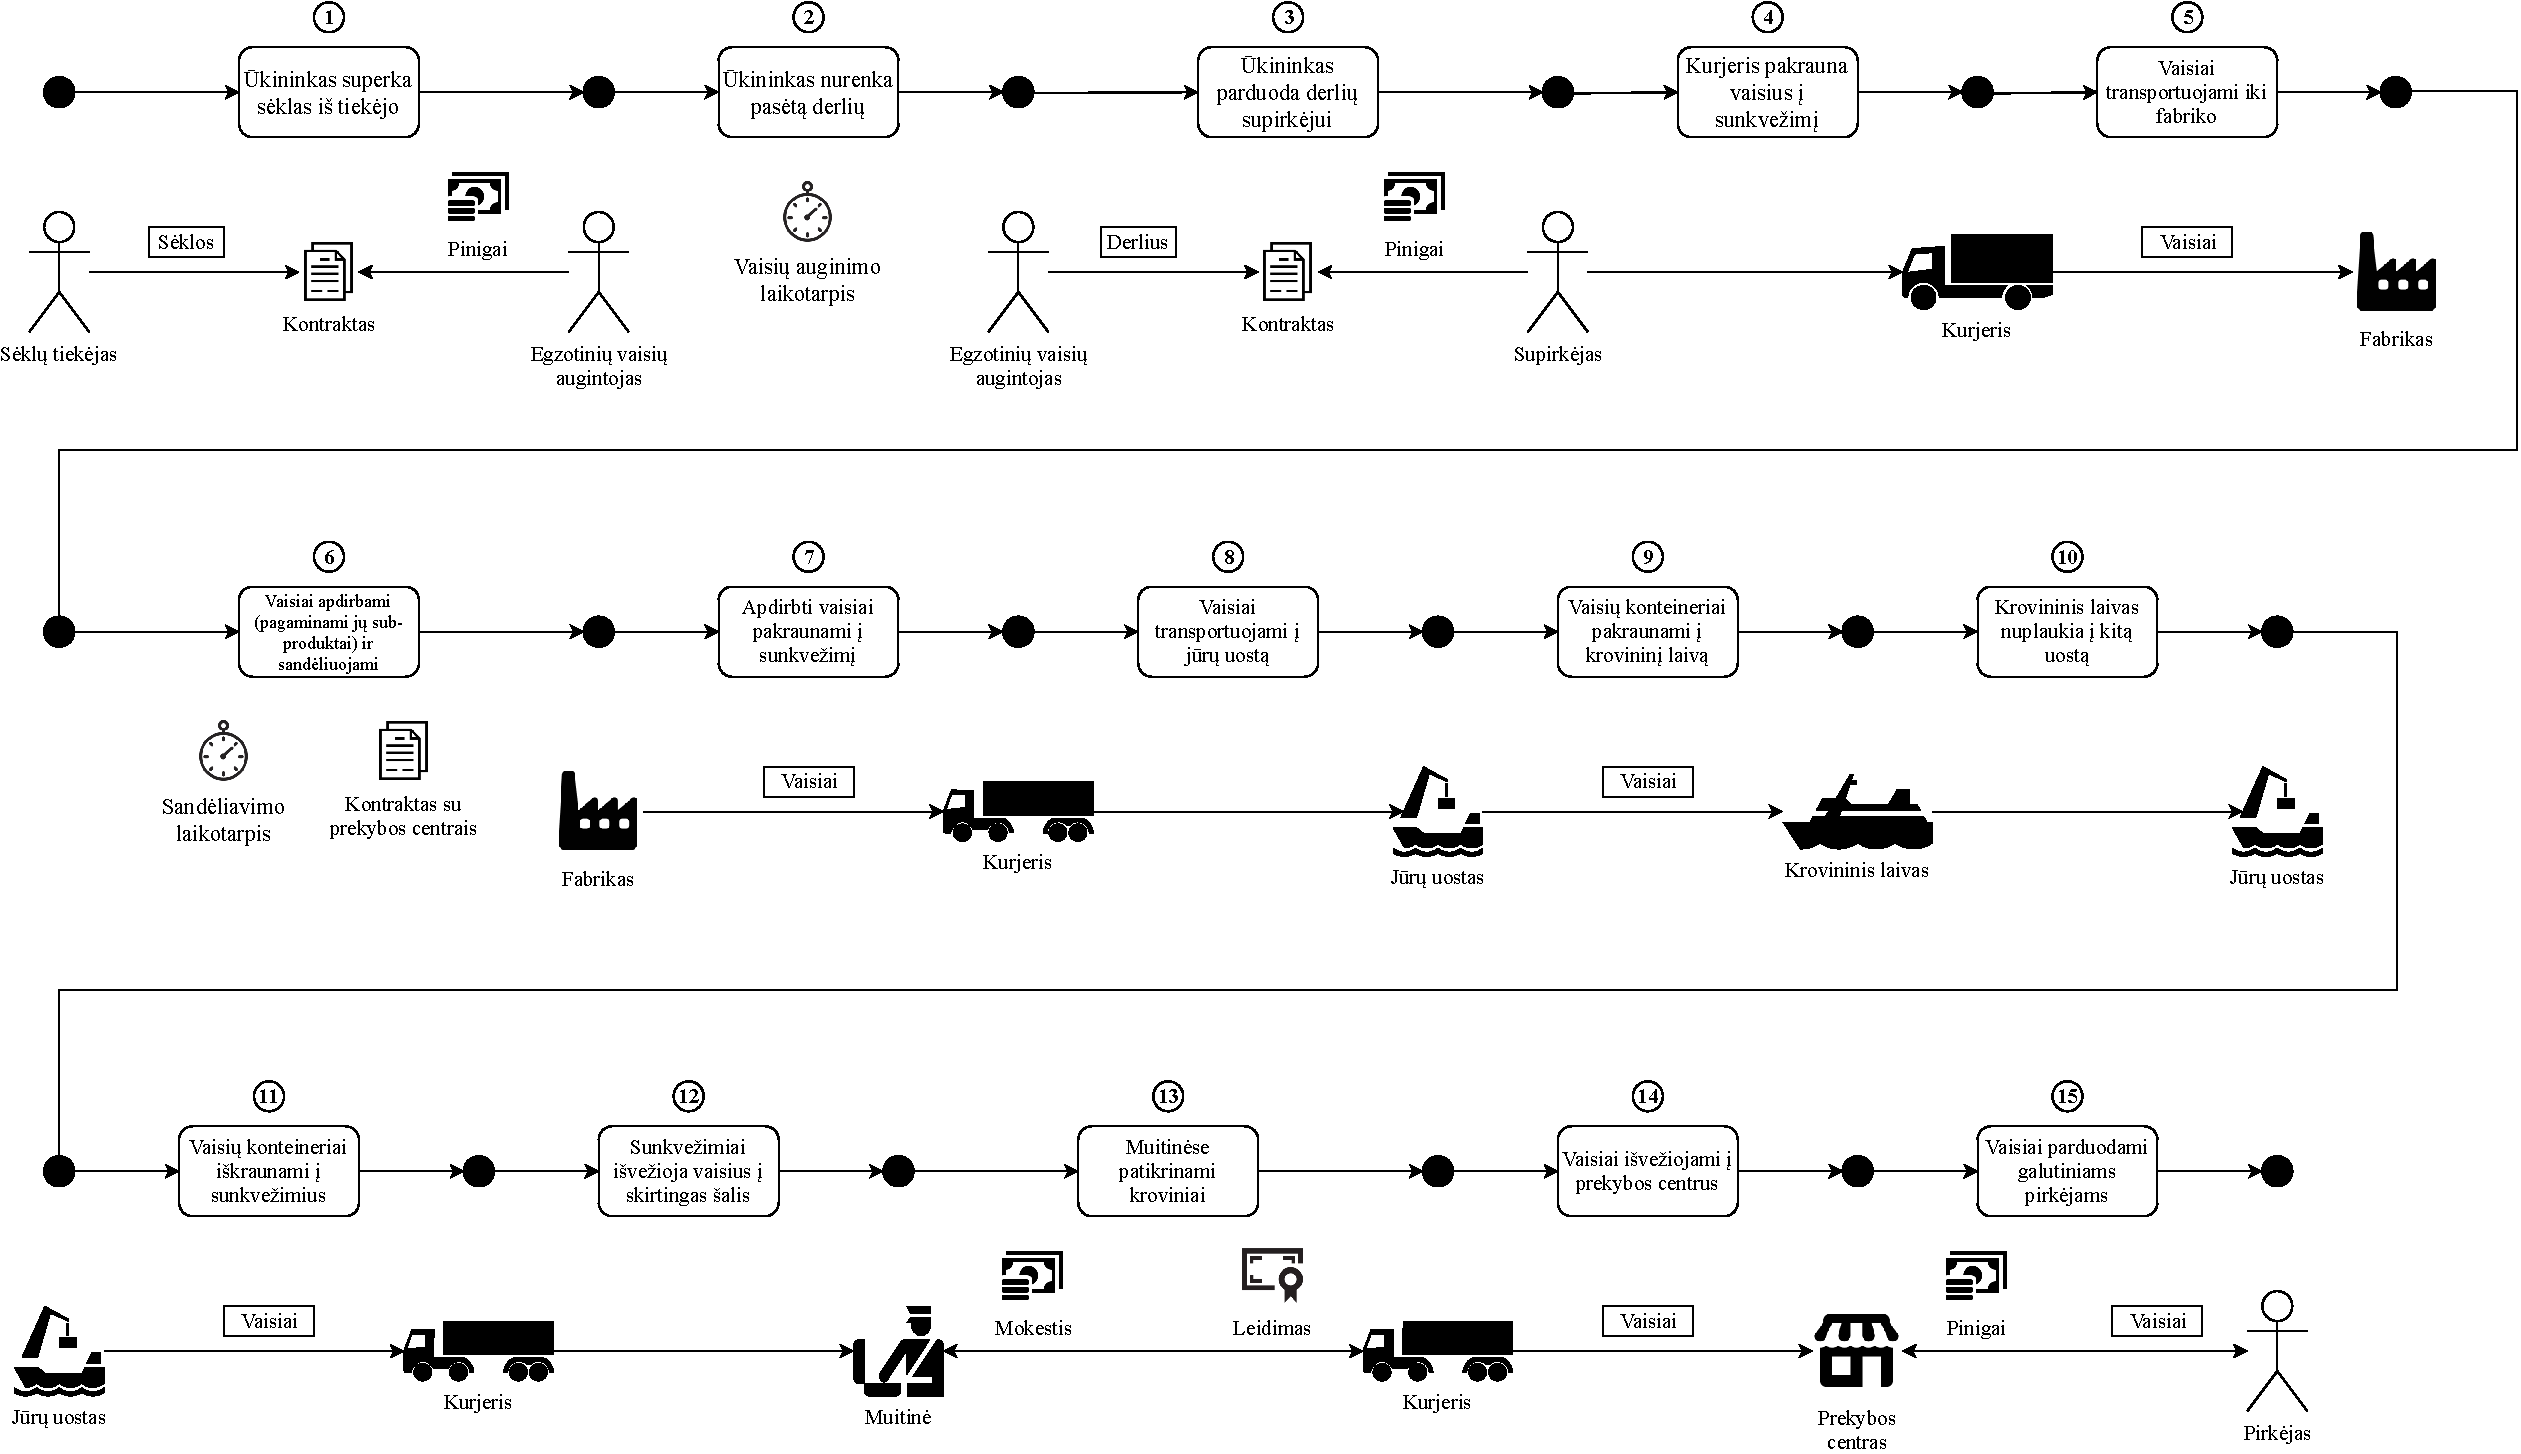
\includegraphics[scale=0.4]{images/supply-chain-horizontal}
    \caption{Įprasta tiekimo grandinė}
\end{figure}

% Prieduose gali būti pateikiama pagalbinė, ypač darbo autoriaus savarankiškai
% parengta, medžiaga. Savarankiški priedai gali būti pateikiami ir
% kompaktiniame diske. Priedai taip pat numeruojami ir vadinami. Darbo tekstas
% su priedais susiejamas nuorodomis.